% !TeX root = ../sustechthesis-example.tex

\chapter[强化学习案例legged\_gym库]{强化学习案例legged\_gym库}

% \section[强化学习案例legged\_gym库]{强化学习案例legged\_gym库\cite[p1]{Rudin_Hoeller_Reist_Hutter_2021}}

% \textcolor{red}{\small
% 这部分展示legge\_gym库关于ANYmal-c的训练代码,主要关注整个训练流程、奖励函数的设计、对Isaac-API的使用、地形设计、训练课程设计等与论文中提到的概念对应...}

\section[legged\_gym工程文件结构]{legged\_gym工程文件结构\cite[p1]{Rudin_Hoeller_Reist_Hutter_2021}}

\begin{figure}
  \centering
  \caption{\emph{legged\_gym} 整体工程文件结构}
  \label{fig:legged_gym_overal_structure}
  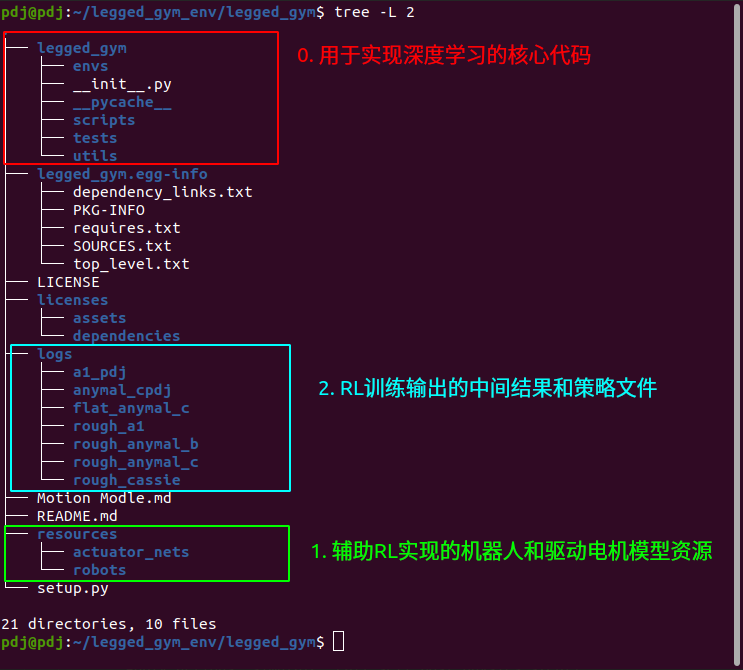
\includegraphics[width=1.0\linewidth]{legged_gym_overal_structure.png}
\end{figure}


\subsection[\emph{legged\_gym}工具包]{\emph{legged\_gym}工具包}
\begin{figure}
  \centering
  \subcaptionbox{\emph{legged\_gym} project structure\label{fig:legged_gym_structure}}
  {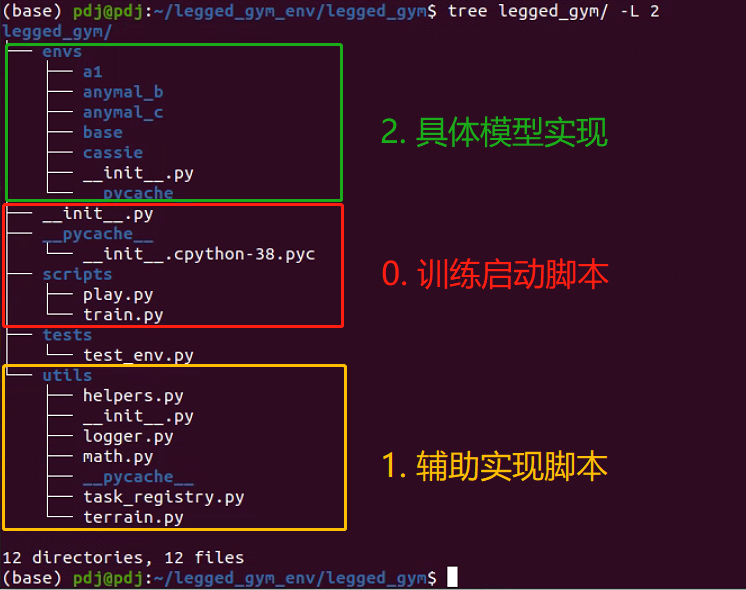
\includegraphics[width=0.43\linewidth]{legged_gym_structure.png}}
  \subcaptionbox{\emph{legged\_gym/envs} folder structure\label{fig:legged_gym_envs_structure}}
  {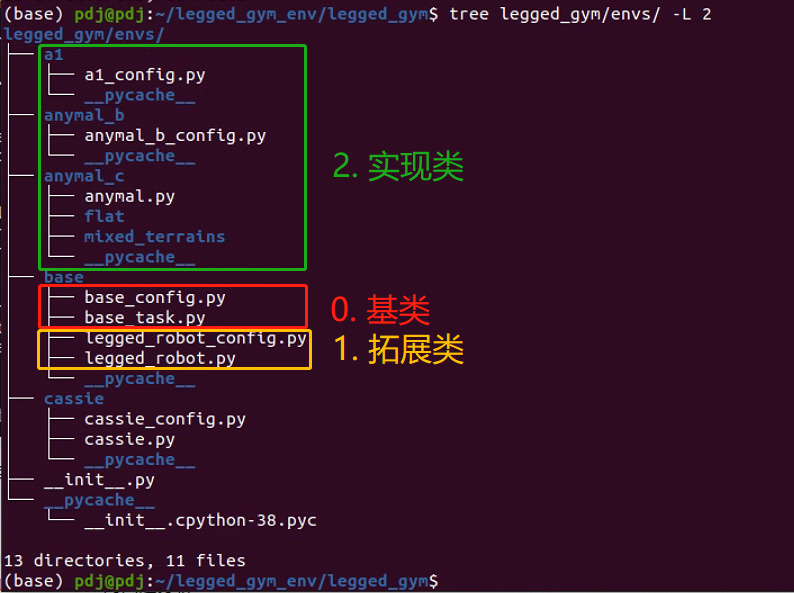
\includegraphics[width=0.46\linewidth]{legged_gym_envs_structure.png}}
\end{figure}


\subsection[从Isaac仿真环境中获取信息]{从Isaac仿真环境中获取信息}

\begin{figure}
  \centering
  \caption{\emph{function: \_init\_buffers} 这个函数处理了来自仿真环境中的数据;初始化了计算会用到的原始信息和将会生成的相关信息的内存空间;设置了关节点的位置偏移和PD增益。}
  \label{fig:legged_function_init_buffers}
  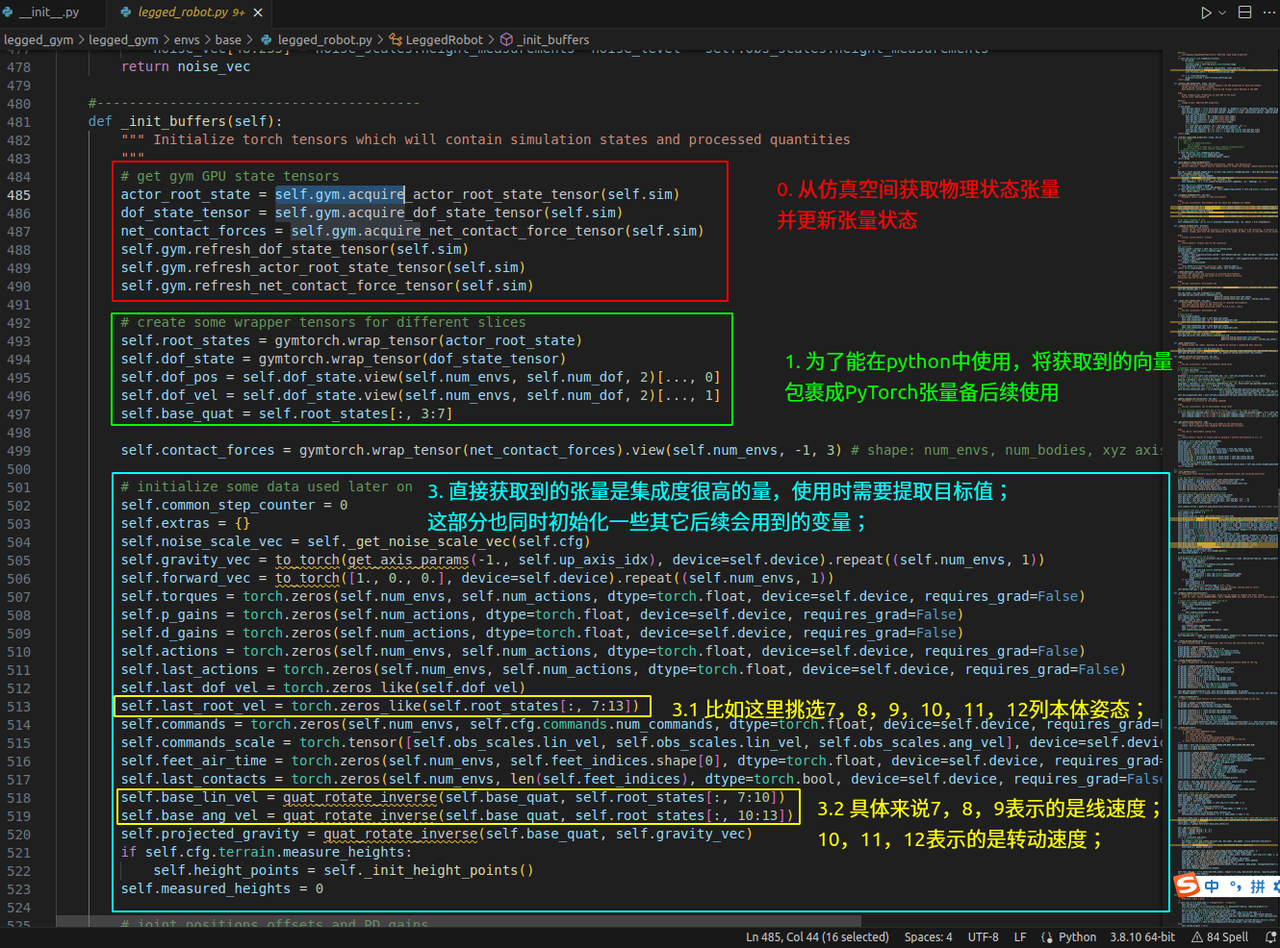
\includegraphics[width=1.0\linewidth]{legged_function_init_buffers.png}
\end{figure}










\section[LeggedRobot类]{LeggedRobot类}
在\emph{legged\_gym}中用于足式机器人的仿真核心类就是\emph{LeggedRobot},它位于\emph{../legged\_gym/legged\_gym/envs/legged\_robot.py}文件中。下面将介绍它内部核心实现函数。

\subsection[LeggedRobot.step函数]{LeggedRobot.step函数}
在整个LeggedRobot类中\emph{step}函数是一个提纲挈领性的函数,它调用其余各个部分函数组件实现仿真的循环。外部函数对LeggedRobot类的激活就是通过调用其中的\emph{step}函数实现的。在\emph{legged\_gym}工程中\emph{step}函数的调用出现在这几个地方:\begin{enumerate}
  \item legged\_gym/legged\_gym/envs/base/base\_task.py中的\emph{BaseTask}类;
  \item legged\_gym/legged\_gym/scripts/play.py中的\emph{play}函数;
  \item legged\_gym/legged\_gym/scripts/test\_env.py中的\emph{test\_env}函数;
\end{enumerate}

\begin{figure}
  \centering
  \caption[LeggedRobot.step函数]{LeggedRobot.step函数}
  \label{fig:legged_function_step}
  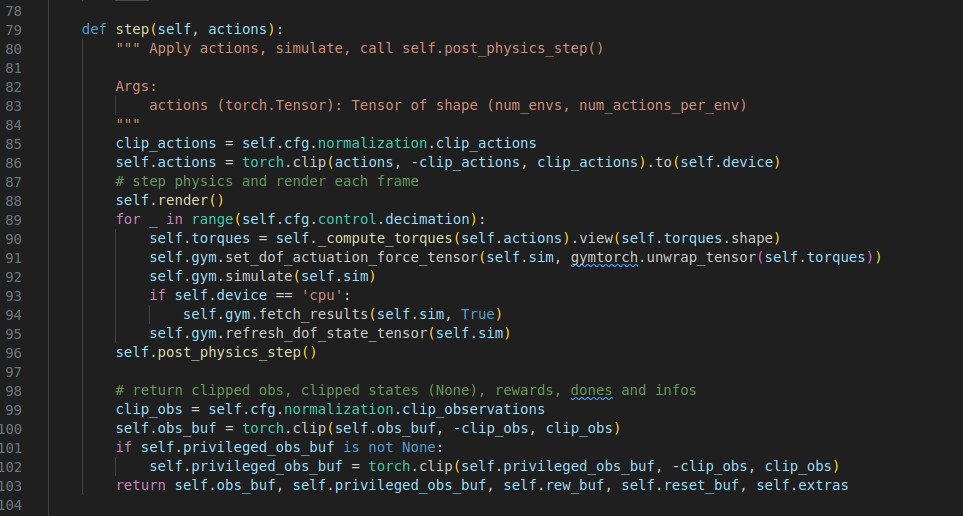
\includegraphics[width=1.0\linewidth]{legged_function_step.png}
\end{figure}

如图所示,\emph{step}函数的功能主要通过调用一下几个函数实现:\begin{enumerate}
  \item \emph{self.render};
  \item \emph{self.compute\_torques};
  \item \emph{self.gym.set\_dof\_actuation\_force\_tensor};
  \item \emph{self.gym.simulate};
  \item \emph{self.gym.fetch\_results}
  \item \emph{self.gym.refresh\_dof\_state\_tensor};
  \item \emph{self.post\_physics\_step};
\end{enumerate}

这其中比较关于仿真环境的\emph{self.gym.xxx}我们暂时不讨论,下面主要关注这三个:\emph{self.render};\emph{self.compute\_torques};\emph{self.post\_physics\_step}。

\subsection[self.render函数]{self.render函数}

\subsection[self.compute\_torques函数]{self.compute\_torques函数}

\subsection[self.post\_physics\_step函数]{self.post\_physics\_step函数}











